% !TEX root = template.tex
\section{Function}

First, we obtain GO annotations~\cite{gene_ontology} for both our family proteins and the entire SwissProt database. To have a more complete representation, we then expanded these GO annotations by parsing the ontology tree~\cite{obo_parser} and adding the ancestor GO terms of each initially found GO term. In order to calculate the enrichment of each GO term in our family compared to the ones found in the SwissProt database, we used Fisher's exact test~\cite{fisher_test}. We used a $2 \times 2$ contingency table where rows indicated the presence or absence of a GO term and columns differentiated between proteins within and outside our domain family (Table~\ref{tab:contingency}). 
\begin{table}[h!]
    \centering
    \small
    \begin{tabular}{lccc}
        \toprule
         & Protein in family & \multicolumn{2}{c}{Protein not in family} \\
        \\
        \midrule
        Has GO term & $a$ & \multicolumn{2}{c}{$b$} \\
        No GO term & $c$ & \multicolumn{2}{c}{$d$} \\
        \bottomrule
    \end{tabular}
    \caption{Contingency table}
    \label{tab:contingency}
\end{table}
For each GO term, we tested two hypotheses. Under the null hypothesis, the proportion of proteins annotated with that given GO term in our domain family equals the proportion in the full SwissProt dataset. We evaluated this against two alternative hypotheses: a right-tailed test to detect enrichment (higher proportion in our family than in SwissProt) and a two-tailed test to detect any significant difference in proportions (either higher or lower). The enrichment value was then calculated as:
$$
\dfrac{family\_proportion}{swissprot\_proportion}
$$
We generated a word cloud visualization using the enriched terms (where $p < 0.05$ for both $p_{\text{two-tailed}}$ and $p_{\text{right-tailed}}$ tests) weighted by their enrichment value (Fig.~\ref{fig:go-wordcloud}). Furthermore, we reported the most enriched branches of the ontology tree based on the enriched terms. For each GO term, we parsed the ontology tree~\cite{obo_parser} up to the root and added the GO term itself as an enriched child to each found ancestor. After this process, we selected only branches - which we defined as the immediate parent of a GO term, or the GO term itself in case of a root term - that had more than $2$ enriched children and a maximum depth of $3$ to filter for high-level terms. A selection of $10$ of these branches, ranked by their cumulative significance score $S = \sum -\log_{10}(p_{\text{two-tailed}})$ calculated across all child terms, can be seen in Table~\ref{tab:go_terms}.


\begin{figure*}[h!]
    \centering
    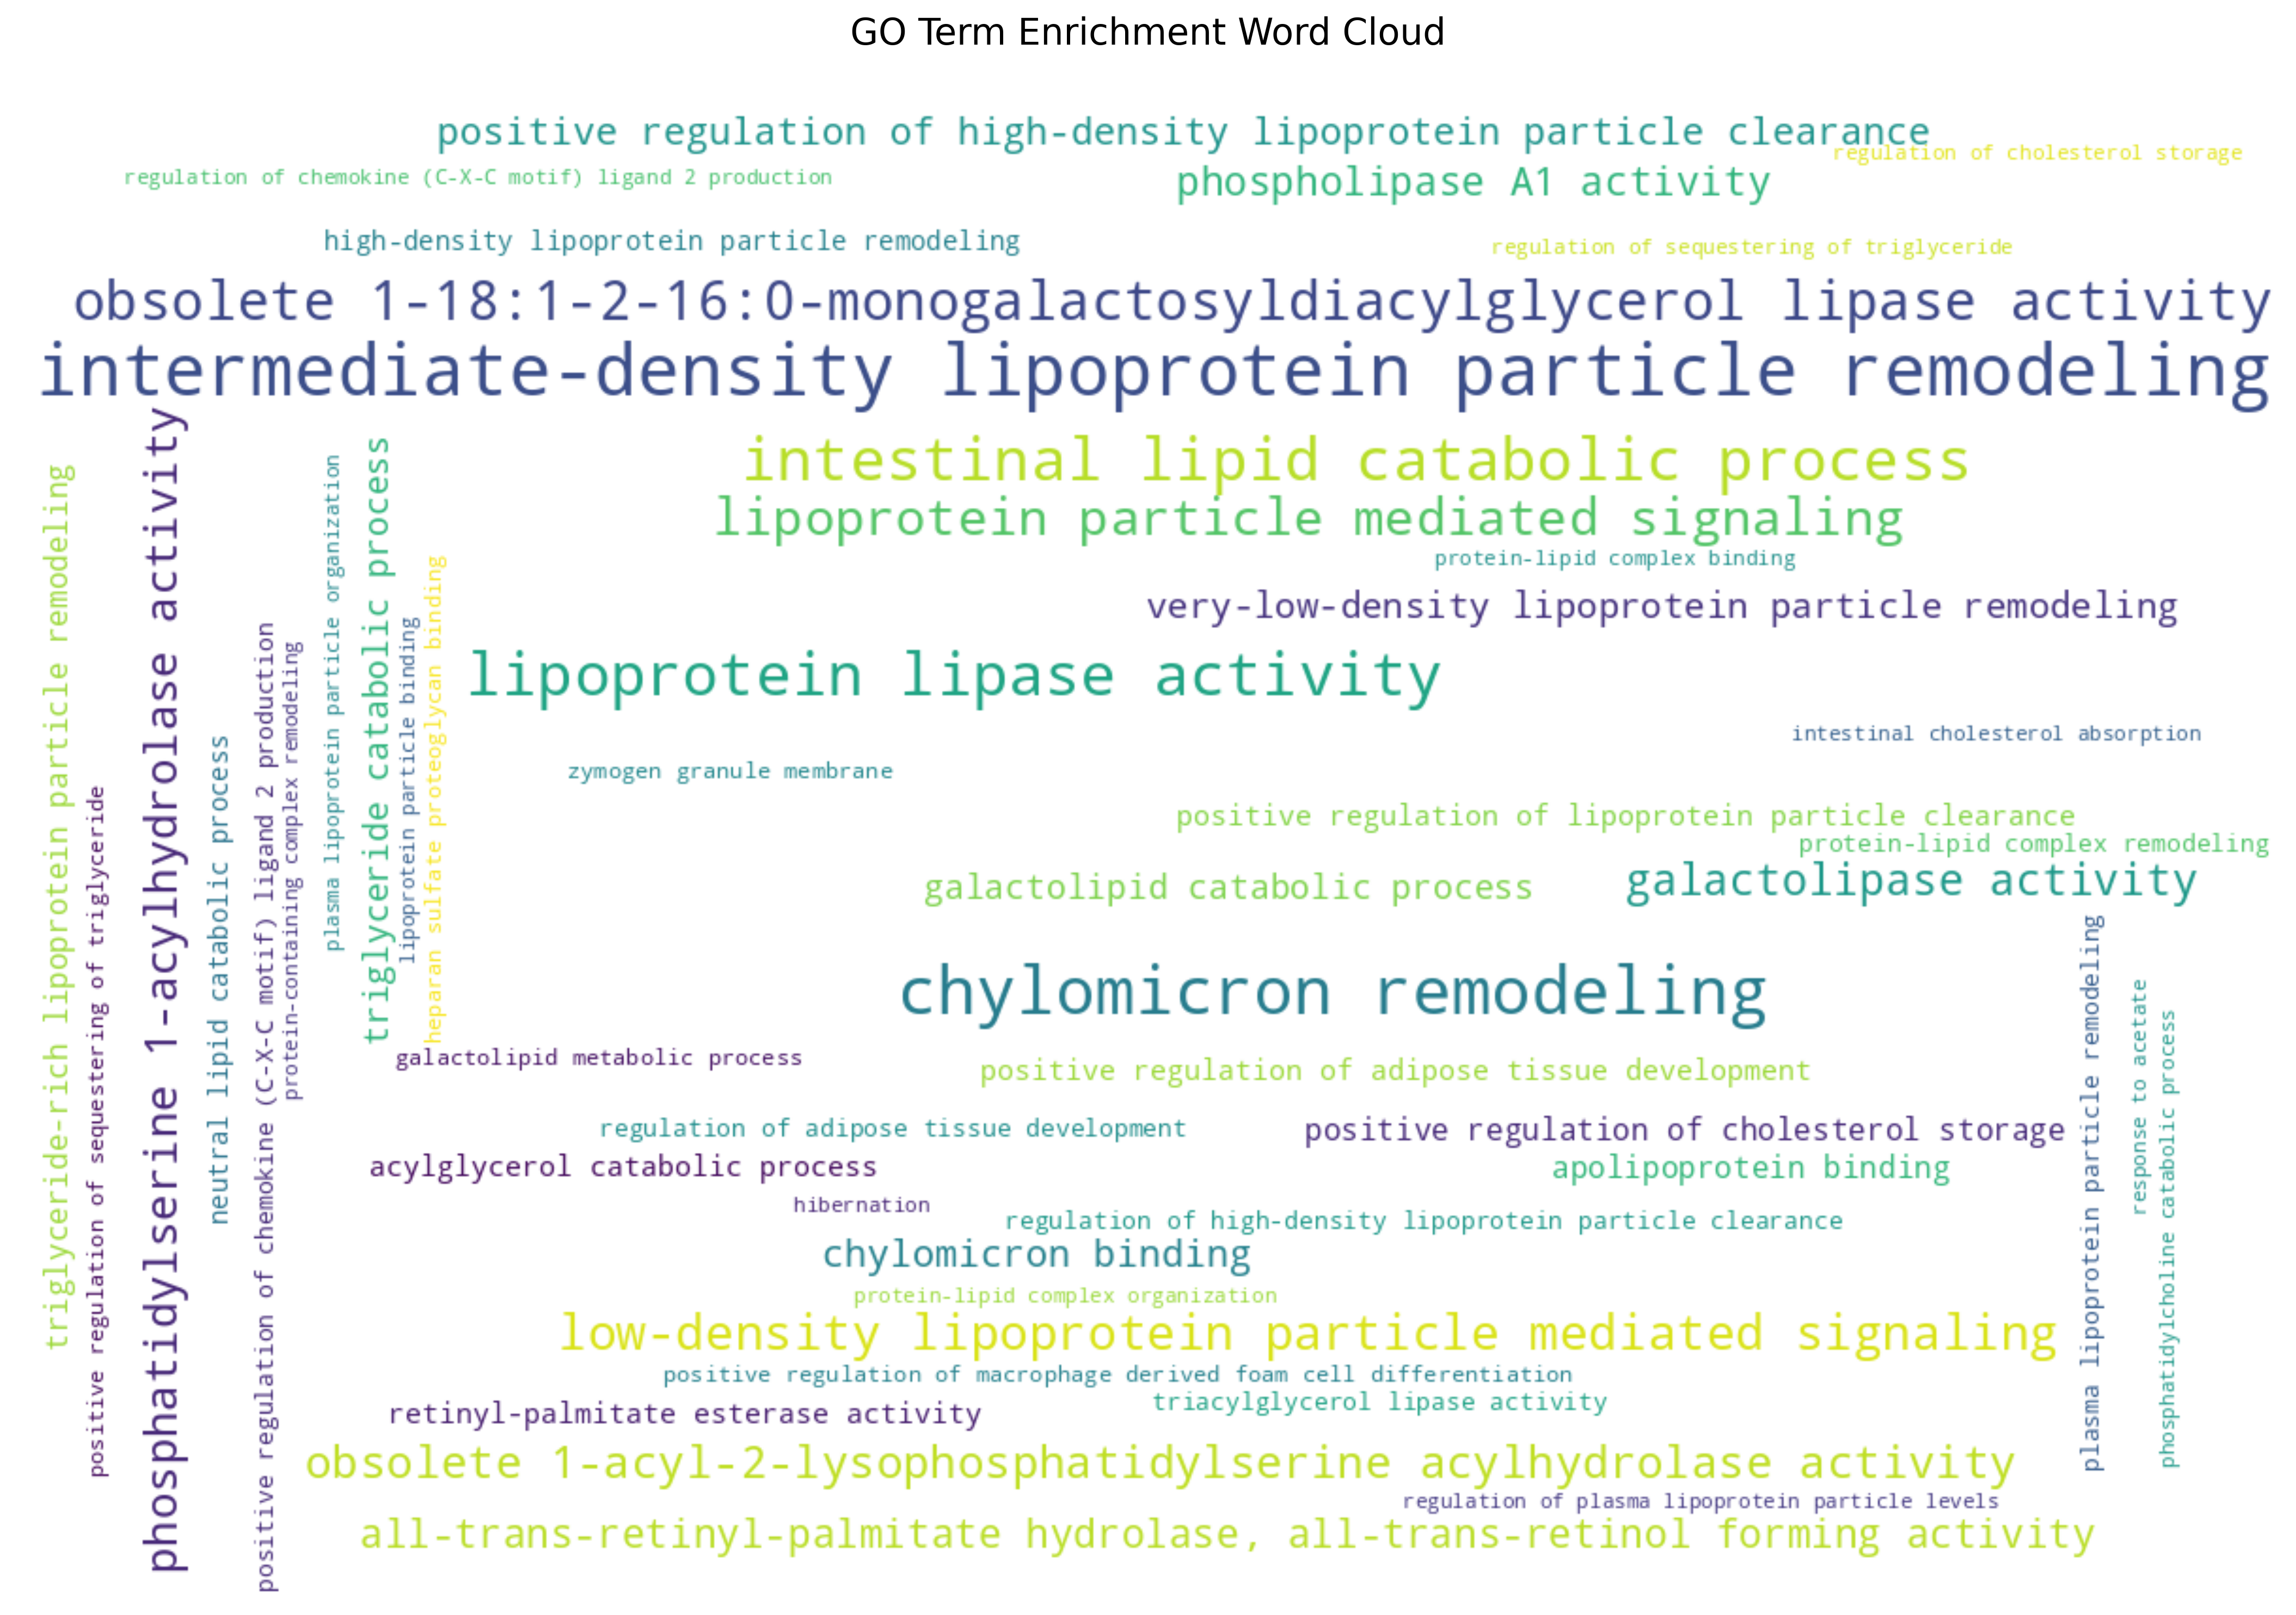
\includegraphics[width=0.8 \textwidth]{images/go_enrichment_wordcloud.png}
    \caption{Word cloud visualization of enriched GO terms. The size of each term represents its relative frequency or significance, with larger text indicating higher enrichment. Terms are related to lipoprotein metabolism, lipase activity, and various cellular processes.}
    \label{fig:go-wordcloud}
\end{figure*}